\begin{activity}{Estimating Crustal Heat Production from Seismic Velocity}

\section*{Purpose}
Thermal conductivity can be measured directly on a hand sample, and gravity, magnetics, and seismic velocity can all be estimated remotely at depth. Heat production cannot -- there is no field survey that tells you $A(z)$ directly. This activity asks whether seismic velocity, which \emph{can} be estimated at depth almost everywhere, can stand in as a proxy for heat production, which can't. It can, to a real and useful degree -- but pushing that proxy all the way to a testable prediction exposes a genuine, unresolved tension between two entirely reasonable ways of estimating the same quantity.

\section*{Learning Outcomes}

By the end of this activity, you should be able to:
\begin{itemize}
  \item Explain why heat production is harder to estimate at depth than density, susceptibility, or resistivity.
  \item Evaluate a real scientific critique of a proposed geophysical proxy relationship, and identify when a change of variable (not new data) resolves it.
  \item Use real velocity-depth data and an empirical velocity-heat production relationship to estimate a terrane's radiogenic crustal heat flow.
  \item Test that estimate against an independent constraint -- conservation of energy -- and reason about which of two disagreeing methods deserves more trust, and why.
\end{itemize}

\section*{Geological Context}
Density, magnetic susceptibility, electrical resistivity, and seismic velocity can all, in principle, be estimated at depth from a surface survey -- that is the entire premise of applied geophysics. Heat production cannot: it has no directly observable geophysical field of its own. Rybach and \v{C}erm\'{a}k proposed a workaround decades ago -- since seismic velocity depends on bulk mineralogy and heat production depends on trace radioactive element concentrations, and both broadly track a rock's felsic-to-mafic character, velocity might serve as an indirect proxy for heat production, remotely sensed the way heat production itself cannot be.

Fountain (1986) pushed back hard: plotted directly, $A$ against $V_p$ is extremely scattered -- visually close to no relationship at all. This activity works through both Fountain's objection and a resolution to it, using two Australian terranes with very different histories: the \textbf{Macquarie Arc}, a Palaeozoic magmatic arc within the Lachlan Orogen, and the \textbf{Yilgarn Craton}, an Archean shield.

\section*{Tasks}
\begin{questions}

  \question{Linear or Log? Revisiting Fountain's Critique}

  Below is measured heat production plotted against P-wave velocity for both terranes, first in linear space, then in $\log_{10}$ space with the fitted relationship $\log_{10}A = m_0(V_p-6.0)+m_1$ overlaid.

  \begin{figure}[h]
      \centering
      
\includegraphics[width=0.85\textwidth]{figures/13_vp_vs_heat_production.pdf}
      \caption{Heat production vs.\ $V_p$, linear space -- Macquarie Arc and Yilgarn Craton.}
      \label{fig:linear_scatter}
  \end{figure}

  \begin{figure}[h]
      \centering
      
\includegraphics[width=0.85\textwidth]{figures/14_vp_vs_log_heat_production.pdf}
      \caption{$\log_{10}A$ vs.\ $V_p$, same data, with the fitted terrane-specific relationships.}
      \label{fig:log_scatter}
  \end{figure}

  \begin{enumerate}[label=(\alph*)]
    \item Looking only at Figure~\ref{fig:linear_scatter}, would you say Fountain had a point?
    \answerbox[1.5cm]

    \item Now look at Figure~\ref{fig:log_scatter}. Has the underlying data changed, or just how it's displayed?
    \answerbox[1.5cm]

    \item Heat production is approximately log-normally distributed. Why would that fact alone explain why the same data looks convincing in one space and hopeless in the other?
    \answerbox[2.5cm]
  \end{enumerate}

  \question{Universal Relationship?}

  The two terranes' fitted relationships are:
  \[
    \text{Macquarie Arc: } \log_{10}A = -0.727\,(V_p-6.0) + 0.551, \qquad
    \text{Yilgarn Craton: } \log_{10}A = -1.193\,(V_p-6.0) + 0.695.
  \]

  \begin{enumerate}[label=(\alph*)]
    \item Which terrane's heat production is more sensitive to velocity -- that is, which has the steeper slope?
    \answerbox[1.5cm]

    \item The global fit across all measured terranes gives a slope of $-0.888$, between these two. Is "one global relationship" a good description of what's actually going on, or is it closer to an average of many genuinely different local relationships?
    \answerbox[2cm]
  \end{enumerate}

  \question{Does Sample Size Matter?}

  Fountain's original critique was based on a global compilation. The figure below shows $r^2$ against sample size $N$ for 322 well-constrained terranes worldwide.

  \begin{figure}[h]
      \centering
      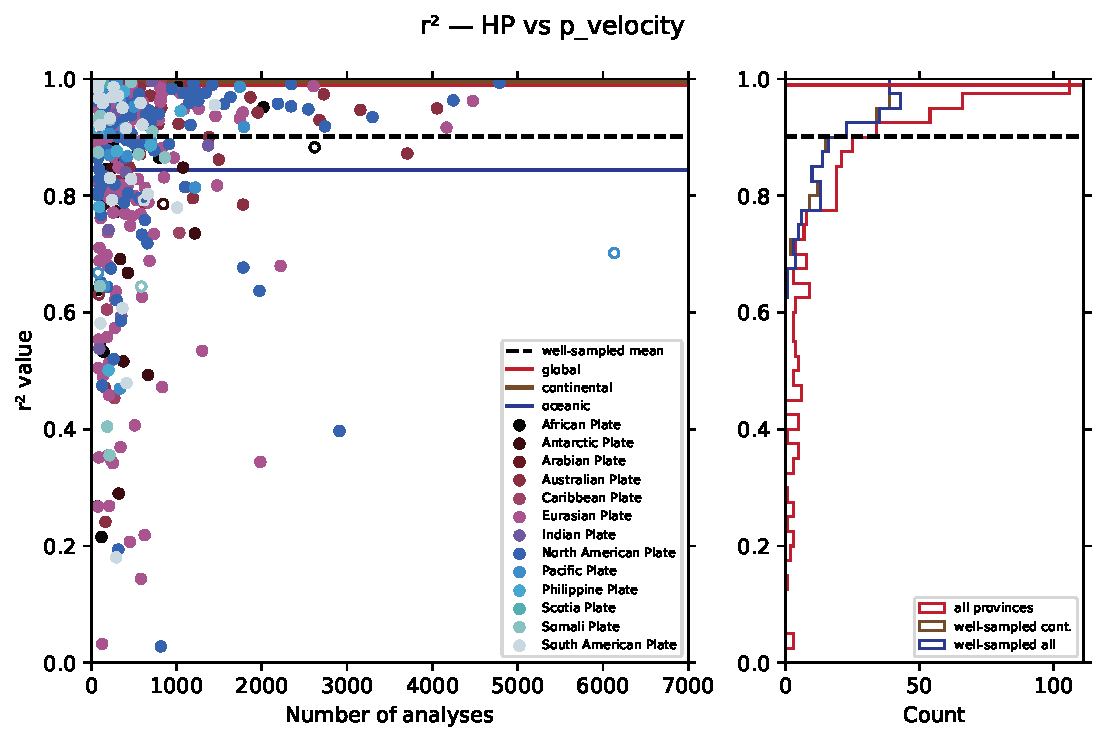
\includegraphics[width=0.8\textwidth]{figures/hp_prov_rsq_p_velocity.pdf}
      \caption{Goodness of fit ($r^2$) vs.\ sample size, across 322 terranes.}
      \label{fig:funnel}
  \end{figure}

  \begin{enumerate}[label=(\alph*)]
    \item Describe the shape of this plot. Does the scatter in $r^2$ stay constant as $N$ grows, or change?
    \answerbox[2cm]

    \item If Fountain's compilation included many terranes with only a handful of samples each, how might that alone have made the relationship look weaker than it really is, without any of the log-space issue from Question 1?
    \answerbox[2.5cm]
  \end{enumerate}

  \question{From Velocity to Heat Production}

  Table~\ref{tab:velocity_depth_stats} gives median $V_p$ in 5~km depth bins for both terranes, from a real crustal velocity model (AuSREM). For each bin, you will convert $V_p$ into a heat production estimate and accumulate it into a crustal radiogenic heat flow.

  Working in $\log_{10}$ space is faster: compute
  \[
    \log_{10}A = m_0(V_p-6.0)+m_1
  \]
  first, then 
  \[
    A=10^{\log_{10}A}\, ,
  \]
  then multiply by the bin's thickness $\Delta z$ (in \si{km}) to get that bin's contribution to heat flow, in mW/m$^2$ --- the units work out directly, with no conversion factor needed, because $\SI{1}{\mu W.m^{-3}} \times \SI{1}{km} = \SI{1}{mW.m^{-2}}$.

  \textbf{Worked example (first row, Macquarie Arc):} at $V_p=6.02$,
  \[
    \log_{10}A = -0.727(6.02-6.0)+0.551 = 0.537\, ,
  \]
  so
  \[ 
    A=10^{0.537}= \SI{3.44}{\mu W.m^{-3}}\, .
  \]
  Over the \SI{5}{km} bin, this contributes $3.44\times5=17.2$~\si{mW.m^2}. The Yilgarn Craton row is done the same way, using its own $m_0$ and $m_1$.
  \begin{table}[h]
    \caption{P-wave velocity statistics by depth interval for each terrane.}
    \label{tab:velocity_depth_stats}
    \begin{tblr}{
        colspec = {crccccX[c]},
        row{6-14,Z} = {ht=2.5em},
        hline{1,4,5,15,16,Z} = {solid},
        hline{6-14,17-25} = {dashed},
        vline{1,8} = {solid},
        vline{6} = {5-14,16-25}{solid},
        vline{7} = {1-3}{5-14,16-25}{dashed},
    }
        & & \SetCell[c=3]{c}{$V_p$} & & \\
        \SetHline{3-5}{0.5pt}
        Depth & N & Median & Mean & Std & $\log_{10} A$ & $A$ \\
        \SetHline{1}{0.5pt}
        \SetHline{3-5}{0.5pt}
        \si{km} & & \SetCell[c=3]{c}{\si{km.s^{-1}}} & & \si{\mu W.m^{-3}}\\
        \SetCell[c=7]{c}{\emph{Macquarie Arc}} \\
        0--5 & 87 & 6.02 & 5.91 & 0.28 & $-0.727\,(6.02-6.0)+0.551 = 0.537$ & $10^{0.537}=3.44$ \\
        5--10 & 87 & 6.18 & 6.16 & 0.13 & & \\
        10--15 & 87 & 6.31 & 6.32 & 0.13 & & \\
        15--20 & 87 & 6.47 & 6.48 & 0.11 & & \\
        20--25 & 87 & 6.62 & 6.63 & 0.09 & & \\
        25--30 & 87 & 6.87 & 6.87 & 0.10 & & \\
        30--35 & 86 & 7.10 & 7.10 & 0.13 & & \\
        35--39.2 & 81 & 7.49 & 7.47 & 0.29 & & \\
        40--42.6 & 48 & 7.65 & 7.63 & 0.25 & & \\
        & & & & & & $q_{\mathrm{rad}} =$ \\
        \SetCell[c=7]{c}{\emph{Yilgarn Craton}} \\
        0--5 & 256 & 6.04 & 6.03 & 0.20 & $-1.193\,(6.04-6.0) + 0.695 = 0.647 $ & $10^{0.647}=4.436$ \\
        5--10 & 256 & 6.13 & 6.16 & 0.15 & 0.540 & 3.47 \\
        10--15 & 256 & 6.33 & 6.32 & 0.16 & 0.301 & 2.00 \\
        15--20 & 253 & 6.54 & 6.53 & 0.13 & 0.051 & 1.24 \\
        20--25 & 253 & 6.67 & 6.72 & 0.18 & -0.104 & 0.787 \\
        25--30 & 253 & 6.94 & 6.98 & 0.20 & -0.426& 0.375 \\
        30--34.7 & 252 & 7.32 & 7.36 & 0.29 & -0.880 & 0.132 \\
        35--38.3 & 184 & 7.79 & 7.81 & 0.20 & -1.44 & 0.036 \\
        40--41.8 & 73 & 7.88 & 7.90 & 0.16 & -1.55 & 0.028\\
        & & & & & & $q_{\mathrm{rad}} =$ \\
    \end{tblr}
\end{table}

  \begin{enumerate}[label=(\alph*)]
    \item Complete the table: fill in $\log_{10}A$, $A$, and each bin's contribution, then sum each terrane's column to get $q_\text{rad,median}$.
    \answerbox[1cm]
    \FloatBarrier

    \item Which terrane's crustal column contributes more heat flow by this estimate? Does that match what you'd have predicted from the slopes in Question 2 alone, or does the shape of the velocity profile with depth also matter?
    \answerbox[2.5cm]
  \end{enumerate}

  \question{The Log-Normal Correction}

  The fitted relationship predicts the \emph{median} $A$ at a given $V_p$ -- but \emph{heat production} is an additive, volumetric quantity, so the physically relevant value for the integral you just computed is the \emph{mean}, not the median. Because $A$ is log-normally distributed, the mean is always larger than the median, by a factor
  \[
    K \approx 10^{1.151 \sigma_{10}^2},
  \]
  where $\sigma_{10}$ is the scatter of $\log_{10}A$ about the fitted line. Measured directly from each terrane's own data: $\sigma_{10}=0.247$ ($K=1.175$) for Macquarie Arc, and $\sigma_{10}=0.342$ ($K=1.364$) for Yilgarn Craton.

  \begin{enumerate}[label=(\alph*)]
    \item Multiply your two sums from Question 4 by the appropriate $K$ to get the corrected, mean-based radiogenic heat flow estimate for each terrane.

    \vspace{0.5em}
    Yilgarn Craton: \numberbox[1.5cm]\ \si{mW.m^{-2}}
    \qquad\qquad 
    Macquarie Arc: \numberbox[1.5cm]\ \si{mW/m^{-2}} \\
    \vspace{0.5em}

    \item Which terrane's estimate changed more in absolute terms? Why, given the two $K$ values?
    \answerbox[2cm]
  \end{enumerate}

  \question{A Paradox?}

  Real heat flow measurements exist for both terranes.

  \begin{center}
  \begin{tabular}{lccc}
    \toprule
    & Sites & Mean observed $q$ (\si{mW.m^2}) & Median observed $q$ (\si{mW.m^2}) \\
    \midrule
    Macquarie Arc   & 48 & 71.2 & 70.3 \\
    Yilgarn Craton  & 66 & 37.8 & 37.1 \\
    \bottomrule
  \end{tabular}
  \end{center}

  In steady state, observed heat flow is the sum of everything generated in the crust above the measurement plus whatever is still arriving from the mantle: $q_\text{observed} = q_\text{rad} + q_\text{mantle}$, so $q_\text{mantle} = q_\text{observed} - q_\text{rad}$.

  \begin{enumerate}[label=(\alph*)]
    \item For each terrane, using your corrected (mean-based) $q_\text{rad}$ from Question 5, compute the implied mantle heat flow $q_\text{mantle}$.
    \answerbox[2.5cm]

    \item Is either result physically possible? What would a negative $q_\text{mantle}$ actually mean?
    \answerbox[2cm]

    \item Two independent, individually reasonable methods -- a velocity-based proxy calibrated against real rock samples, and a direct energy-conservation argument -- disagree here, sometimes severely. Which do you trust more, and why? What does each method actually depend on that the other doesn't?
    \answerbox[3cm]

    \item This activity opened by asking whether heat production could be estimated the way density, susceptibility, or resistivity can be. Having worked through this, what's your answer now -- and what, specifically, makes heat production harder?
    \answerbox[2.5cm]
  \end{enumerate}

\end{questions}

\section*{Key Ideas}

\textbf{A relationship can be real and still look like noise, if you're looking in the wrong space.} Fountain's critique wasn't wrong about what he saw -- linear-space $A$-$V_p$ data genuinely is scattered. It was wrong about what that scatter meant, because it didn't account for heat production's log-normal distribution.

\textbf{An empirical proxy relationship is only as trustworthy as the data used to build it -- and it can be genuinely strong without being universal.} Different terranes show different, real, well-constrained slopes; treating any single fit (even the well-supported global one) as a universal law discards information the data itself is offering.

\textbf{When two independently-motivated methods disagree, ask what each one is actually constrained by.} A velocity-based proxy is constrained only by the rock samples used to calibrate it -- nothing stops it from predicting an impossible total. An energy-conservation argument is constrained by the whole system having to balance, and cannot produce a physically impossible answer without signalling that fact directly, as a negative flux. That asymmetry, not just "geophysics being more careful," is why the energy-balance constraint deserves more trust when the two disagree.

\end{activity}